\documentclass{ximera}

%\colorlet{penColor}{blue!50!black} % Color of a curve in a plot
%\colorlet{gridColor}{gray!50} % Color of grid in a plot
%\colorlet{background}{white} % Color of the page
\newcommand{\ddx}{\frac{d}{dx}}
\newcommand{\dydx}{\frac{dy}{dx}}
\newcommand{\dd}[2][]{\frac{d #1}{d #2}}


\outcome{What is a limit?}

\outcome{What is a one-sided limit?}

\outcome{Understand the difference between evaluating functions and
  taking limits of functions.}

\outcome{When does a limit not exist?}

\outcome{Interpert limits and one-sided limits.}

\outcome{Calculate limits from a graph or state that the limit does not exist.}

\outcome{Estimate limits using nearby values.}

\title{The definition of limits}

\begin{document}

\begin{abstract}
  Let's see if we can think about what limits allow us to do.
\end{abstract}
\maketitle


Sometimes we have functions that are not defined at certain
points. For example, consider

\[
f(x) = \frac{x^2 - 3x + 2}{x-2}.
\]

You may be tempted to divide by $x^2 - 3x + 2$ by $x-2$, and conclude
that our function is equal to $x-1$. However this is not true!

\[
f(x) = x-1 \qquad\text{only when $x\ne 2$,}
\]

the function $f(x)$ is \textbf{undefined} when $x= 2$, since if we
attempt to compute $f(2)$ we find

\[
f(2) = \frac{2^2-3\cdot 2+2}{2-2} = \frac{0}{0}\qquad\text{which is  undefined}.
\]

There are other types of functions that are undefined at given points. 

\begin{question}
  Below we have a collection of functions and points. Which
  function(s) is/are defined at the given point?
\begin{solution}
\begin{multiple-choice}
\choice[correct]{$f(x) = \sqrt{x}$ at $x= 0$}
\choice{$f(x) = \frac{1}{x}$ at $x= 0$}
\choice{$f(x) = \ln(x)$ at $x=0$}
\choice{$f(x) = \sin^{-1}(x)$ at $x=2$}
\choice{$f(x) = \frac{x^2-3x+2}{x-2}$ at $x=2$}
\end{multiple-choice}
\end{solution}
\end{question}


Continuing on with the example of 

\[
f(x) = \frac{x^2 - 3x + 2}{x-2},
\]

let's see a plot of this function:

\begin{image}
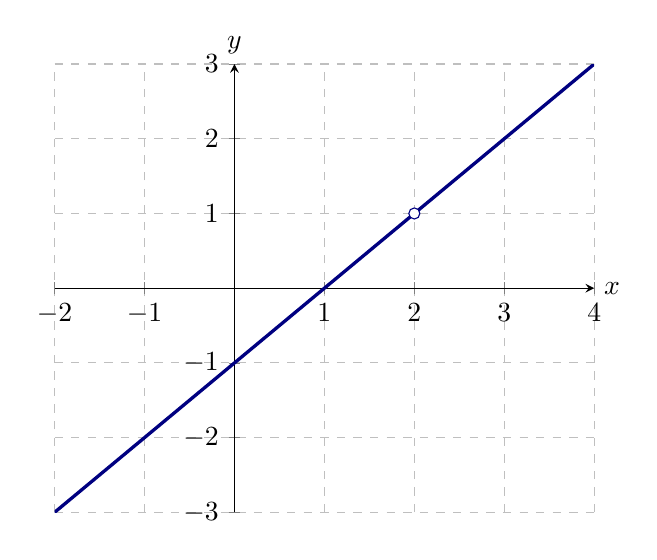
\begin{tikzpicture}
  \colorlet{penColor}{blue!50!black} % Color of a curve in a plot
\colorlet{gridColor}{gray!50} % Color of grid in a plot
\colorlet{background}{white} % Color of the page
	\begin{axis}[
            domain=-2:4,
            axis lines =middle, xlabel=$x$, ylabel=$y$,
            every axis y label/.style={at=(current axis.above origin),anchor=south},
            every axis x label/.style={at=(current axis.right of origin),anchor=west},
            grid=both,
            grid style={dashed, gridColor},
            xtick={-2,...,4},
            ytick={-3,...,3},
          ]
	  \addplot [very thick, penColor, smooth] {x-1};
          \addplot[color=penColor,fill=background,only marks,mark=*] coordinates{(2,1)};  %% open hole
        \end{axis}
\end{tikzpicture}
\end{image}

The fact that $f(x)$ is not defined at the point $x=2$ is denoted by
the open circle. You can think of this as a ``hole'' in the
function. After looking at the plot, someone with a cavalier attitude
might just say $f(2) = 1$, \textbf{but this is not true!}

What is correct is that if you name a number close to but not equal to
$1$, we can find a point $x_0$ close to but not equal to $2$, so that
$f(x_0)$ is closer to $1$ than your number. Let's write this more
abstractly:

\begin{definition}
The notation:

\[
\lim_{x\to a} f(x) = L
\]

means that for every number close to but not equal to $L$, we can find
a point $x_0$ close to but not equal to $a$, so that $f(x_0)$ is
closer to $L$ than your number.
\end{definition}




\begin{question}
  What is the correct answer to this question?

  \begin{solution}
    \begin{multiple-choice}
      \choice[correct]{Correct answer}
      \choice{First Distractor}
      \choice{Second Distractor}
      \choice{Third Distractor}
    \end{multiple-choice}  
  \end{solution}
\end{question}

What other questions do you have about this lecture?
\begin{free-response}
\end{free-response}

\end{document}
